
%(BEGIN_QUESTION)
% Copyright 2015, Tony R. Kuphaldt, released under the Creative Commons Attribution License (v 1.0)
% This means you may do almost anything with this work of mine, so long as you give me proper credit

Read and outline the ``Differential (87) Current Protection'' section of the ``Electric Power Measurement and Control'' chapter in your {\it Lessons In Industrial Instrumentation} textbook.  Note the page numbers where important illustrations, photographs, equations, tables, and other relevant details are found.  Prepare to thoughtfully discuss with your instructor and classmates the concepts and examples explored in this reading.

\underbar{file i03031}
%(END_QUESTION)




%(BEGIN_ANSWER)


%(END_ANSWER)





%(BEGIN_NOTES)

Differential current protection (ANSI/IEEE code 87) is based on Kirchhoff's Current Law, which states the algebraic sum of all currents entering and exiting a node must be equal to zero.  If we measure the amount of current entering and exiting any electrical component or subsystem and find those currents to be unequal, it means current is traveling along a different route than what the circuit should allow, and that fault needs to be cleared.  Since {\it any} amount of current imbalance is technically abnormal, we may employ 87 relays with high sensitivity and no time delay thus ensuring faster clearing of the fault.

\vskip 10pt

A GFCI (Ground Fault Current Interruptor) power receptacle is an example of differential current protection, tripping on any detected hot/neutral current imbalances down to the milliamp range.

\vskip 10pt

Practical 87 relays have both {\it operate} and {\it restraint} coils, to account for imbalances in current due to CT mismatch, CT inaccuracy, and other factors such as harmonics.  The principle is that the 87 relay will trip if the current mismatch exceeds some percentage of total line current rather than tripping based on a fixed threshold (pickup) value.  Modern microprocessor-based 87 relays may be programmed with any number of nonlinear operate/restraint functions to suit different applications.

\vskip 10pt

The {\it zone of protection} for any protective relay is that span of the power network protected against faults by the relay.  Overcurrent relays have ill-defined zones of protection since they trip on current magnitude alone.  Differential current relays have very well-defined zones of protection bounded by the sensing CTs.  In any protected power system, protection zones should overlap at circuit breakers, to ensure no circuit breaker is left unprotected.  This is why circuit breakers typically have CTs installed at each line and load terminal (6 CTs for a three-phase breaker): to permit zone overlap, with each protective relay connected to the CT(s) on the {\it far side} of the breaker.

\vskip 10pt

87 differential current relays may be used to protect bus systems from internal faults, by connecting all far-side CT secondaries in parallel so their currents will add to the current-sensing relay.  This of course requires the use of perfectly matched CT ratios all around in order to work.

\vskip 10pt

Differential current protection of transformers is challenging, especially for three-phase transformer banks having Wye-Delta or Delta-Wye connections.  The concept is to compare current in each secondary line with the current through each corresponding primary line.  In transformers with phase shift between primary and secondary (e.g. Wye-Delta or Delta-Wye configurations), this means the CTs must be connected in complementary fashion (e.g. Delta-Wye or Wye-Delta).  Modern digital transformer differential relays offer ``CT compensation'' features whereby CTs may be connected identically (e.g. both sets of CTs in Wye configuration) and the transformer's phase shift mathematically compensated for in the relay's software. 

\vskip 10pt

A phenomenon seen with transformers is {\it inrush current} when first energized.  If the transformer's magnetic core is saturated, extra primary current will be drawn that is not reflected in the secondary windings, which may lead to false 87 relay trips.  Equipping the 87 relay to detect harmonic-rich currents which happen to go along with transformer inrush, the relay may be programmed to ignore current imbalances as long as the harmonics persist.





\filbreak

\vskip 20pt \vbox{\hrule \hbox{\strut \vrule{} {\bf Suggestions for Socratic discussion} \vrule} \hrule}

\begin{itemize}
\item{} Explain why CT polarity is critically important in differential current protection circuits.
\item{} Explain why CT polarity is unimportant in 50/51 overcurrent protection circuits.
\item{} Calculate operate coil (OC) and restraint coil (RC) currents in a generator 87 protection circuit given a certain phase current value, and two CT ratios that are slightly mismatched:
\itemitem{} 850 amps $I_{line}$ ; 1200:5 and 1203:5 ratios ; {\it RC1 = 3.54 A ; RC2 = 3.53 A ; OP = 0.0088 A}
\itemitem{} 900 amps $I_{line}$ ; 1000:5 and 1007:5 ratios ; {\it RC1 = 4.50 A ; RC2 = 4.47 A ; OP = 0.0313 A} 
\itemitem{} 720 amps $I_{line}$ ; 800:5 and 801:5 ratios ; {\it RC1 = 4.50 A ; RC2 = 4.49 A ; OP = 0.0056 A} 
\itemitem{} 328 amps $I_{line}$ ; 400:5 and 404:5 ratios ; {\it RC1 = 4.10 A ; RC2 = 4.06 A ; OP = 0.0406 A} 
\item{} If someone installed one of the CTs for a phase backwards (i.e. primary power line passing the wrong way through the CT's center), could the CT still be wired to the 87 relay in such a way that the system will still work?
\item{} Explain in detail what a {\it protection zone} is.
\item{} Explain how a GFCI is a form of 87 protection.
\item{} Explain how protection zones for 87 relays are defined by the placement of the CTs.
\item{} Examine the single-line diagram in LIII showing multiple, overlapping protection zones and explain why the overlap is important by posing a ``thought experiment'' where a certain differential current fault is assumed.
\item{} Examine the photograph taken of a generator bus at Grand Coulee Dam and identify good placements for CTs to be used in a differential current protection scheme.
\item{} Comparing the ``Comprehensive'' versus ``Crude'' transformer differential current protection circuits shown in the LIII textbook, explain how and why they differ from each other.  Specifically, which type(s) of fault would the Comprehensive circuit detect that the Crude circuit could not, and why?
\item{} Explain why Delta-Wye and Wye-Delta transformers pose a challenge for differential current protection.  How, exactly, is this challenge addressed, when using electromechanical relays and when using digital relays?
\end{itemize}












\vfil \eject

\noindent
{\bf Prep Quiz:}

The purpose of a {\it restraining coil} (``RC'') in an electromechanical 87 relay or a {\it restraining element} in a digital 87 relay is to:

\begin{itemize}
\item{} Make the relay more sensitive to faults outside the protection zone
\vskip 5pt 
\item{} Make CT ratios irrelevant so we may use any CT ratios that we wish
\vskip 5pt 
\item{} Add a time-delay function to the relay so it doesn't trip too fast
\vskip 5pt 
\item{} Avoid false trips due to normal, heavy-load conditions
\vskip 5pt 
\item{} Provide a self-calibrating function to the relay
\vskip 5pt 
\item{} Prevent any CT from generating a dangerous voltage if open-circuited
\end{itemize}












\vfil \eject

\noindent
{\bf Prep Quiz:}

Identify the proper pair of current transformers to connect this line-protection 87 relay's inputs:

$$\includegraphics[width=15.5cm]{i03031x01.eps}$$

\begin{itemize}
\item{} A and B
\vskip 5pt 
\item{} A and C
\vskip 5pt 
\item{} A and D
\vskip 5pt 
\item{} B and C
\vskip 5pt 
\item{} B and D
\vskip 5pt 
\item{} C and D
\end{itemize}














\vfil \eject

\noindent
{\bf Summary Quiz:}

Ground Fault Current Interruptors (GFCIs) come equipped with a {\it test switch} designed to test the ground-fault detection capabilities of the unit when pressed.  Sketch your own test switch into the circuit below (complete with any additional components you see fit to add) so that its function may be routinely tested without causing damage or incurring any other risk:

$$\includegraphics[width=15.5cm]{i03031x02.eps}$$

%INDEX% Reading assignment: Lessons In Industrial Instrumentation, differential (87) current protection

%(END_NOTES)


